\part{Appendices}

\phantomsection
\addcontentsline{toc}{chapter}{List of Figures}
\listoffigures
\clearpage{\pagestyle{plain}\cleardoublepage}  % per aggiungere una pagina vuota (se questa è dispari ne aggiunge un'altra ancora)

\phantomsection
\addcontentsline{toc}{chapter}{List of Tables}
\listoftables
\clearpage{\pagestyle{plain}\cleardoublepage}  % per aggiungere una pagina vuota (se questa è dispari ne aggiunge un'altra ancora)

\begingroup
% \let\cleardoublepage\clearpage

\begin{appendices}
\appendix
%\VerbatimInput[fontsize=\scriptsize, baselinestretch=0.9]{Inputfiles/Filename}

\chapter{Appendix 1}
    \begin{figure}[!htb]
        \centering
        \caption[Degree Distribution]{\textbf{Degree Distribution.} The degree distributions of both the drug (a) and target (b) projections (red), compared to those of equivalent random graphs (blue). The last ones were generated with the Erdős-Rényi model\autocite{Erds1959}, keeping the same number of nodes and probability of edge creation (ratio between the actual number of edges and the maximum possible edges) of the network they are compared with.}
        \label{fig:SI_degree_distribution}
        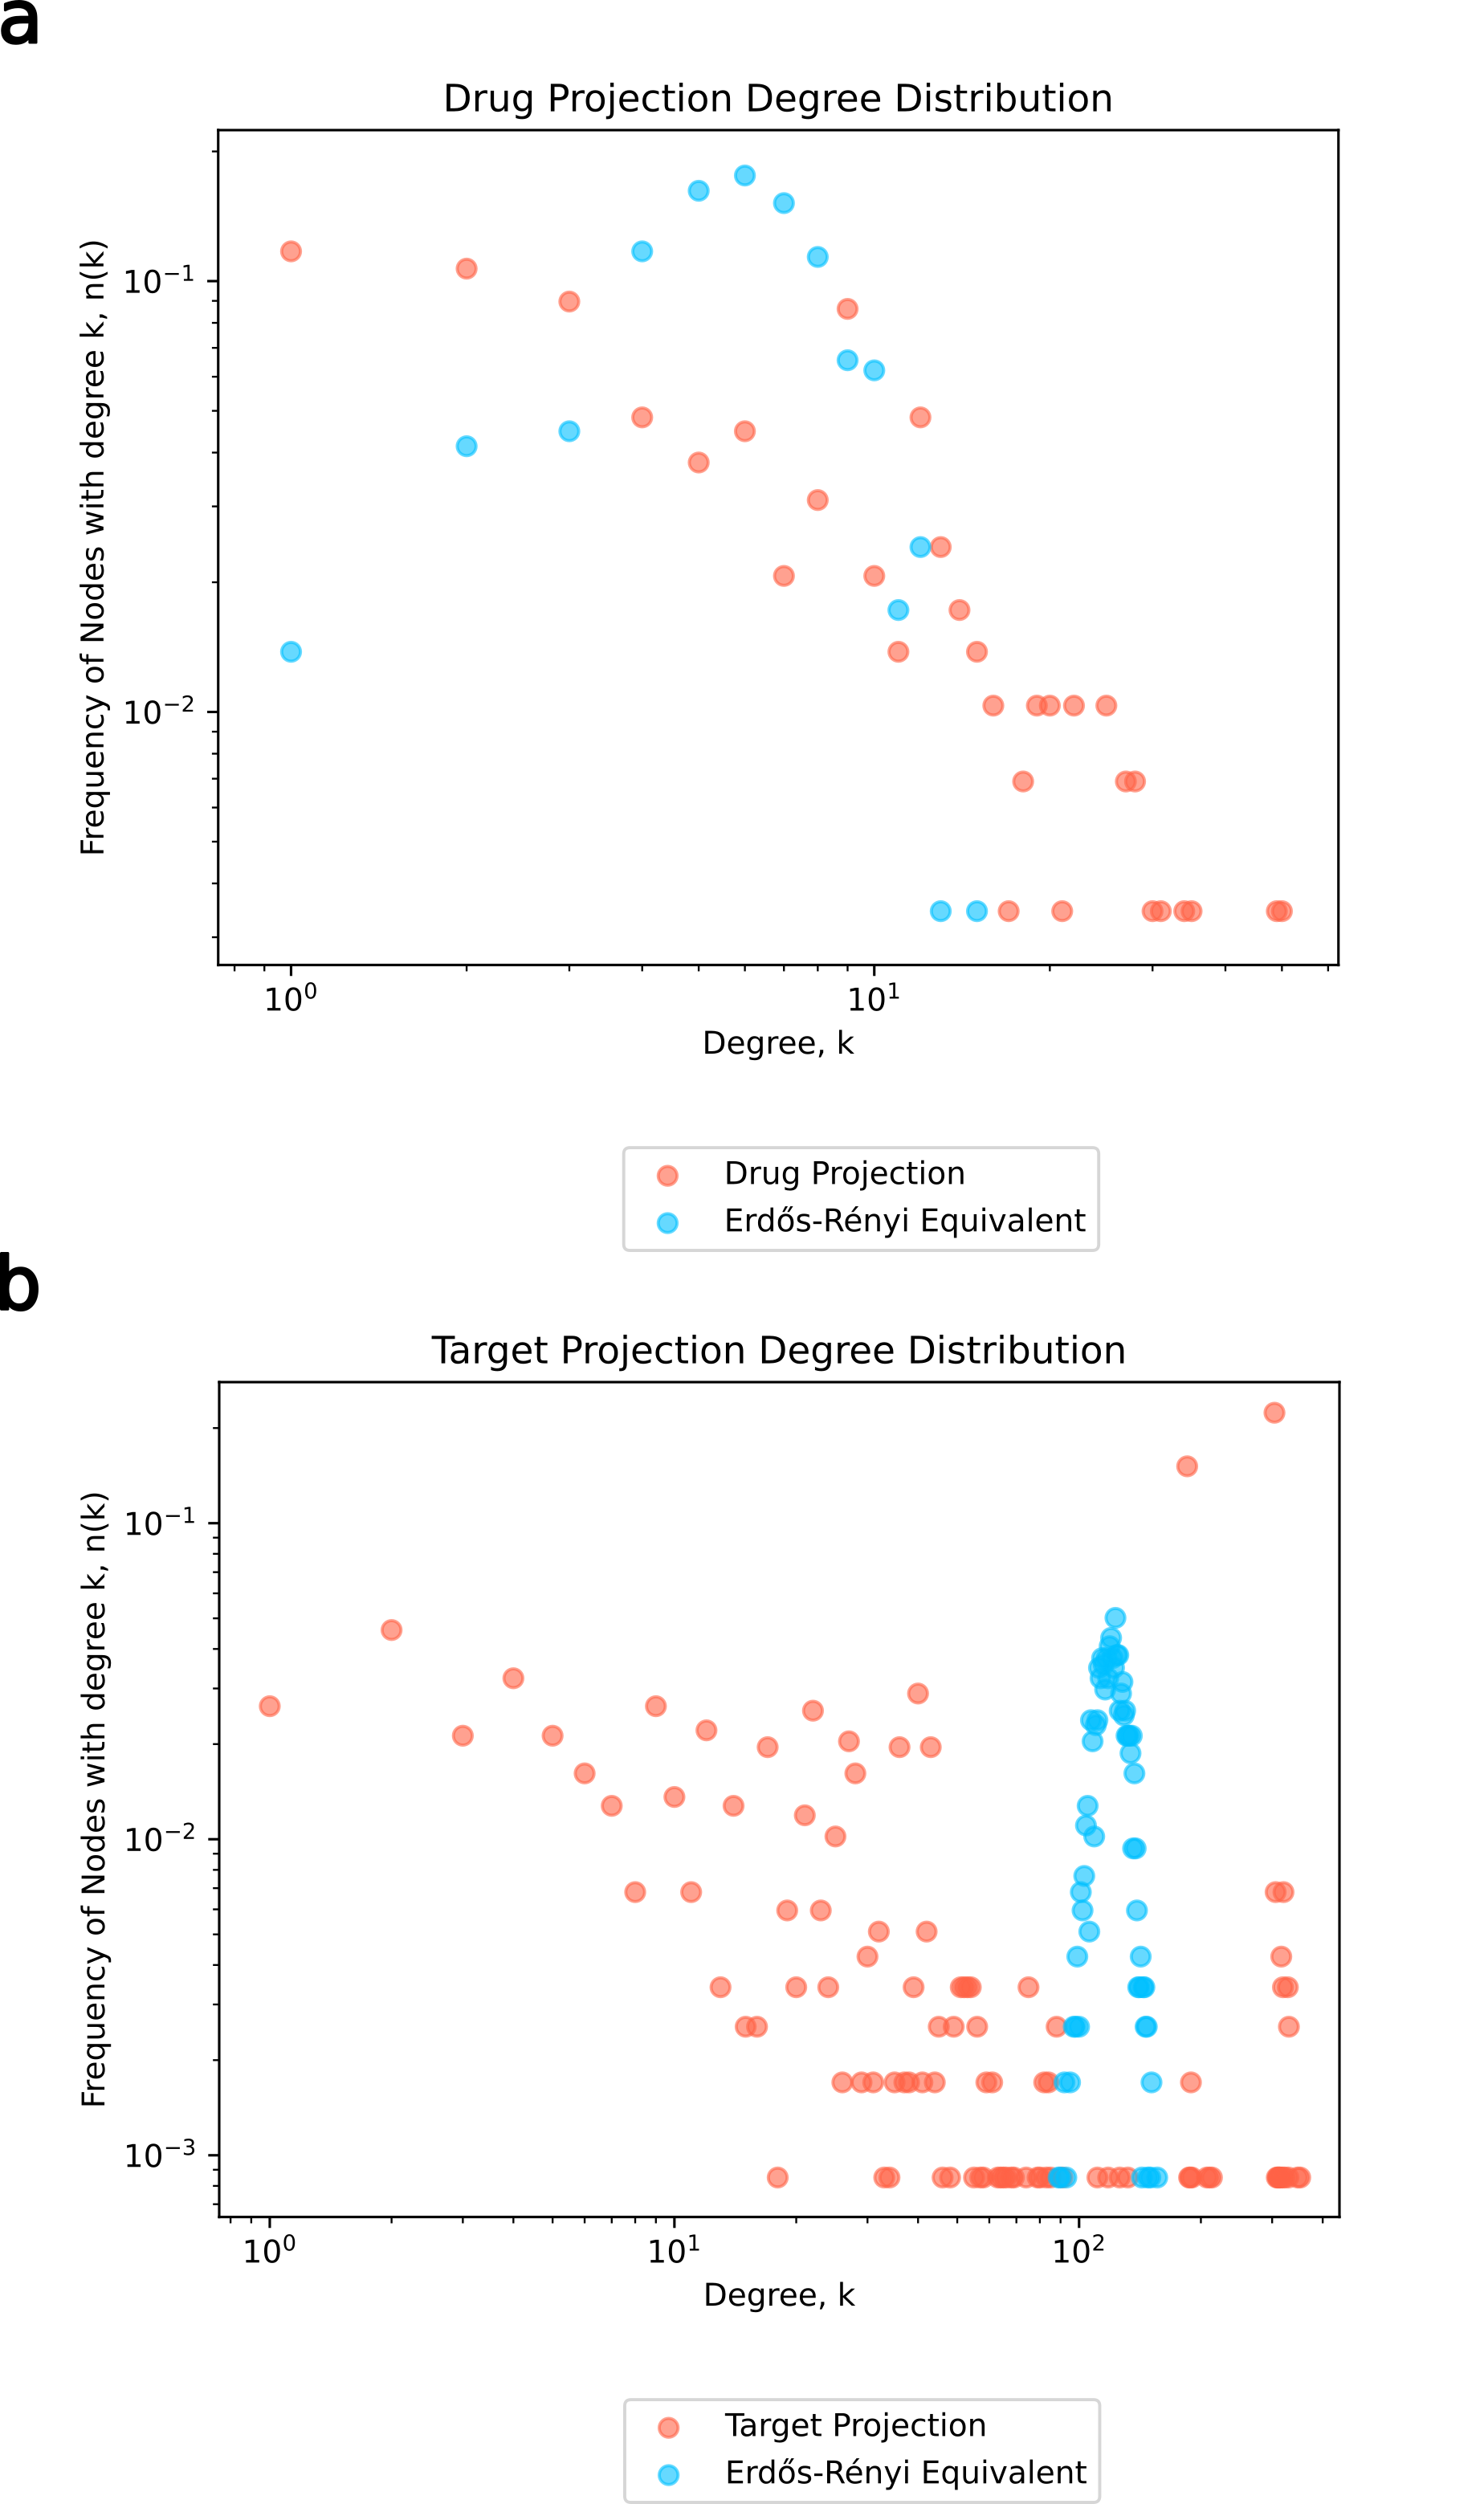
\includegraphics[width=(\textwidth/100)*80]{Images/Project1/SI/Figure_S1.png}
    \end{figure}

    \begin{table}[!htb]
        \footnotesize
        \centering
        \caption[Fittings Evaluation]{\textbf{Fittings Evaluation.} The table provides the log-likelihood and respective p-value for each function fitted on every analyzed network. For the power-law function, the Kolmogorov-Smirnov distance (D) is provided, and the fitting is considered plausible if the respective p-value is at least 0.1.}\label{tab:fittings_evaluation}
        \begin{tabular}{ccccc}
             & \multicolumn{2}{c}{\thead{Drug Projection (Entire)}} & \multicolumn{2}{c}{\thead{Drug Projection}} \\\midrule
             & D & p-value & D & p-value \\\toprule
            Power-Law & 0.07 & 2.4 $\times 10^{-1}$ & 0.05 & 3.3 $\times 10^{-1}$ \\\midrule
             & Likelihood-ratio & p-value & Likelihood-ratio & p-value \\\toprule
            Truncated Power-Law & -0.58 & 2.8 $\times 10^{-1}$ & -8.01 & 6.3 $\times 10^{-5}$ \\\midrule
            Exponential & 0.91 & 6.9 $\times 10^{-1}$ & 15.71 & 6.6 $\times 10^{-2}$ \\\midrule
            Stretched Exponential & -0.42 & 5.8 $\times 10^{-1}$ & -6.80 & 4.8 $\times 10^{-3}$ \\\midrule
            Lognormal & -0.33 & 5.9 $\times 10^{-1}$ & -5.92 & 7.1 $\times 10^{-3}$ \\\bottomrule\bottomrule
             & \multicolumn{2}{c}{\thead{Target Projection (Entire)}} & \multicolumn{2}{c}{\thead{Target Projection}} \\\midrule
             & D & p-value & D & p-value \\\toprule
            Power-Law & 0.22 & 0.0 & 0.06 & 9.5 $\times 10^{-2}$ \\\midrule
             & Likelihood-ratio & p-value & Likelihood-ratio & p-value \\\toprule
            Truncated Power-Law & -329.39 & 0.0 & -9.43 & 1.4 $\times 10^{-5}$ \\\midrule
            Exponential & -349.29 & 1.0 $\times 10^{-21}$ & -3.57 & 5.6 $\times 10^{-1}$ \\\midrule
            Stretched Exponential & -397.78 & 1.66 $\times 10^{-54}$ & -9.27 & 6.6 $\times 10^{-4}$ \\\midrule
            Lognormal & -317.17 & 1.1 $\times 10^{-51}$ & -8.86 & 1.1 $\times 10^{-3}$ \\\bottomrule
        \end{tabular}
    \end{table}

\end{appendices}
\endgroup
% \clearpage{\pagestyle{plain}\cleardoublepage}  % per aggiungere una pagina vuota (se questa è dispari ne aggiunge un'altra ancora)